\documentclass[14pt]{extarticle}

\usepackage[margin=1.2in]{geometry}
\usepackage{longtable}
\usepackage{graphicx} % Required to insert images

\title{\textbf{2D Platformer Engine Documentation}
}
\author{\\ \bf{Main Dev: Nathan Hughes} \\
\\
	\\	Email: nathan1hughes@gmail.com\\
		Github: github.com/sirsharpest \\
		Twitter: @sirsharpest\\
		\\
		\\
		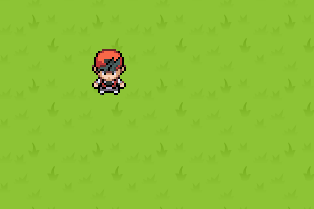
\includegraphics[width=0.75\columnwidth ,height=5cm, keepaspectratio]{tile} 
		\\
		\\
		\\
		\\
		\\
		\\ }
\date{Last edited: \today}

\begin{document}

\maketitle

\clearpage 

\tableofcontents{}
\clearpage

\section{Introduction}
\par
This project is hoping to build a entire 2D game engine that can handle a platformer game akin to the famous Super Mario franchise. 
\\
\\ 
The game that is aiming to use this engine is repetitively simple in itself. Being very vague the game will allow the player to move on two axis to transverse a large tile map. 
\\
\\
The engine will be made using the SFML 2.X library to handle most all of the window, rendering, sound, input and geometry of the game. 

\section{Scope and scale}
\par 
As mentioned previously the end goal of this project is to create a game engine which can be used for a variety of things. As it is created, new challenges and new techniques are encountered, the scope may have to adapt i.e. we may find that it is possible/required to branch out and incorporate additional libraries such as "Boost". 
\\
\\
A highlight the current goals:
\begin{itemize}
	\item{Provide keyboard, mouse and controller support for user input}
		\subitem{\em{In the future we may consider mobile forms of I/O}}
	\item{Read in a plain text document and produce a game map}
	\item{Have basic/rudimentary 2D physics.}
		\subitem{\em{Or use an existing one such as "Box2D"}}
	\item{Handle 2D tile collision}
	\item{Have a (possibly global) solution for holding all references to sprites in memory and reusing them, 
			we don't want duplicated sprites in memory!}
	\item{Saving and storing game data in either XML or JSON}
	\item{Sound/Music engine working correctly}
	\item{Menu system and GUI components}
	\item{Generic item type classes that could be further used for things like "equip-able", "consumable" or 				"Currency"}
\end{itemize} 

The overall project will be considered completed whenever all of this has been implemented and to a high standard! 


\section{Progress Milestones} 
\par 
At current the project has several features implemented and a huge amount left to be done. To provide a somewhat measurable mechanism for progress we will summarise the time/content goals. 

   	\subsection{Milestone 1}
      For this first milestone it would be best to have a very much "proof of concept" build meaning:
      \begin{itemize}
      	
      	\item{Input can be handled {\em easily}  and buttons attached to functionality}
      	\item{Loading of maps can be done as a 2D array hard coded in for testing}
      	\item{Animated sprites are available and can easily be added/loaded in to the global store}
      	\item{Tidy codebase that can be easily edited and added to}
      	\item{Sprite movement along a tile-grid}
      	\item{Keep all movement and calculations relative to delta-time}
      \end{itemize}
      
   	\subsection{Milestone 2}
      This section milestone will aim to practically use the functionality currently implemented, that is to say, a small simple game perhaps "Pick 'n' sticks" or an Asteroids style game would be perfect for this. 
      \\
      \\
Addressing all things created by this goal will push the progress of this game engine into a "Alpha" state 
      \begin{itemize}
      	
      	\item{A small game is produced using implemented features of the engine in its pre-alpha state}
      	\item{A blackbox style of testing will be applied to all code produced for it}
      	\item{Testing will be done on Linux and Windows extensively}
      	\item{A list of issues and annoyances will be produced from both the player and programmer perspective,
      			this list can then be used to perform minor refactors on the code-base }
      \end{itemize}
      

\section{Timeframe}
For each milestone there will be an aimed for date (as these are met/passed, progress reports will follow for that particular milestone), this is currently set as follows:

\begin{longtable}{|c|c|}

\hline
Milestone 1 & 15th April \\
\hline
Milestone 2 & 6th May \\
\hline

\end{longtable}



\end{document}
